% !TeX program = lualatex
% !TeX encoding = UTF-8
% Документ подготовлен для компиляции LuaLaTeX

\documentclass[14pt,a4paper]{extarticle}

% ===== УЛУЧШЕНИЕ ПЕРЕНОСОВ И ТИПОГРАФИКИ =====
\usepackage{microtype}      % микротипографика – уменьшает overfull
\usepackage{icomma}         % перенос чисел с запятой
\setlength{\emergencystretch}{3em}   % разрешить чуть больше растягивать строки
\setlength{\hfuzz}{2pt}              % не показывать overfull до 2pt

% ===== ШРИФТЫ =====
\usepackage{fontspec}
\setmainfont{Times New Roman}[
    BoldFont=Times New Roman Bold,
    ItalicFont=Times New Roman Italic,
    BoldItalicFont=Times New Roman Bold Italic,
    Scale=1.0,
    Ligatures=TeX
]
% Если Times New Roman не установлен – раскомментируйте следующую строку:
% \setmainfont{TeX Gyre Termes}

% ===== РУССКИЙ ЯЗЫК =====
\usepackage[english]{babel}
\babelprovide[import, main]{russian}

% ===== МАТЕМАТИКА =====
\usepackage{amsmath,amsfonts,amssymb}

% ===== ГРАФИКА И ТАБЛИЦЫ =====
\usepackage{graphicx}
\usepackage{float}          % для опции [H] у плавающих объектов
\usepackage{geometry}
\geometry{top=2cm, bottom=2cm, left=3cm, right=1.5cm}
\usepackage{setspace}
\onehalfspacing
\usepackage{indentfirst}
\setlength{\parindent}{1.25cm}
\usepackage{bookmark}
\usepackage{caption}
\captionsetup[table]{justification=raggedright, singlelinecheck=false, labelsep=endash, font=small}
\captionsetup[figure]{justification=centering, labelsep=endash, font=small}

\usepackage{booktabs}
\usepackage{array}
\usepackage{multirow}
\usepackage{hyperref}
\usepackage{enumitem}

\hypersetup{
    colorlinks=true,
    linkcolor=black,
    citecolor=black,
    urlcolor=blue
}

% ===== ЗАГОЛОВКИ =====
\usepackage{titlesec}
\titleformat{\section}
  {\normalfont\fontsize{14}{16}\bfseries\centering}
  {\thesection}{1em}{}
\titleformat{\subsection}
  {\normalfont\fontsize{14}{16}\bfseries}
  {\thesubsection}{1em}{}
\titleformat{\subsubsection}
  {\normalfont\fontsize{14}{16}\bfseries}
  {\thesubsubsection}{1em}{}

\titlespacing*{\section}{0pt}{14pt}{14pt}
\titlespacing*{\subsection}{0pt}{12pt}{12pt}
\titlespacing*{\subsubsection}{0pt}{10pt}{10pt}

% Настройка нумерации страниц: на титульном листе номер не ставится
\pagenumbering{gobble}

% Борьба с вылезанием текста
\usepackage{microtype}
\usepackage{icomma}
\usepackage{ragged2e}
\setlength{\emergencystretch}{5em}      % больше не бойся
\setlength{\hfuzz}{15pt}                % вообще не показывать предупреждения о вылезании <15pt
\sloppy                                % последний довод

\begin{document}

% ==== ТИТУЛЬНЫЙ ЛИСТ ====
\begin{titlepage}
    \centering
    \vspace*{1cm}
    
    {\small МИНИСТЕРСТВО ОБРАЗОВАНИЯ РЕСПУБЛИКИ БЕЛАРУСЬ\\[2pt]
    БЕЛОРУССКИЙ ГОСУДАРСТВЕННЫЙ УНИВЕРСИТЕТ\\[2pt]
    ФАКУЛЬТЕТ ПРИКЛАДНОЙ МАТЕМАТИКИ И ИНФОРМАТИКИ\\[2pt]
    КАФЕДРА МАТЕМАТИЧЕСКОГО МОДЕЛИРОВАНИЯ И АНАЛИЗА ДАННЫХ}
    
    \vspace{3cm}
    
    {\large\bfseries Курсовая работа}
    
    \vspace{1.5cm}
    
    {\Large\bfseries «Анализ финансовой стабильности компаний с помощью алгоритмов машинного обучения»}
    
    \vspace{2cm}
    
    \begin{flushright}
        \begin{tabular}{@{}l@{}}
            Ковалевского Климентия Евгеньевича \\
            студента 3 курса, 7 группы \\
            специальности «Прикладная математика»
        \end{tabular}
    \end{flushright}
    
    \vspace{2cm}
    
    \begin{flushright}
        \begin{tabular}{@{}l@{}}
            \textbf{Научный руководитель:} \\
            В.И. Малюгин \\
            зав. кафедрой ММАД, \\
            доктор экономических наук, \\
            кандидат физ.-мат. наук, \\
            профессор
        \end{tabular}
    \end{flushright}
    
    \vfill
    
    {\large Минск, 2026}
\end{titlepage}

% После титульного листа включаем нумерацию
\clearpage
\pagenumbering{arabic}
\setcounter{page}{2}

\tableofcontents
\clearpage

\clearpage

% ==== ВВЕДЕНИЕ ====
\section*{ВВЕДЕНИЕ}
\addcontentsline{toc}{section}{ВВЕДЕНИЕ}

В условиях современной экономики, характеризующейся высокой динамикой 
и нестабильностью, обеспечение финансовой стабильности компаний 
является одной из ключевых задач как для самих предприятий, 
так и для финансовых институтов, регуляторов и инвесторов. 
Финансовая стабильность выступает индикатором устойчивости компании 
к внешним и внутренним шокам, её способности выполнять обязательства 
и сохранять платежеспособность в долгосрочной перспективе. Традиционные 
подходы к оценке финансового состояния, основанные на анализе 
бухгалтерской отчётности и расчёте финансовых коэффициентов, хотя и 
остаются фундаментом анализа, часто оказываются недостаточными для 
комплексной и оперативной оценки из-за большого объёма данных, 
сложности взаимосвязей и наличия скрытых закономерностей.

В этой связи актуальным становится применение методов машинного 
обучения (\textit{Machine Learning --- ML}), которые позволяют 
автоматизировать процесс анализа, выявлять нелинейные зависимости, 
классифицировать компании по уровню риска и строить прогнозные модели 
на основе исторических данных. Использование \textit{ML}-алгоритмов 
даёт возможность перейти от описательной аналитики к предиктивному 
моделированию, что особенно важно для задач риск-менеджмента, 
кредитного скоринга и раннего предупреждения кризисных явлений.

Целью данного курсового проекта является построение статистических 
кредитных рейтингов с помощью методов машинного обучения.

Для достижения данной цели решаются следующие задачи:
\begin{enumerate}
    \item подготовить обзор существующих методов построения статистических кредитных рейтингов, 
    определить цели и задачи исследования;
    \item разработать математическое описание используемых в работе моделей и алгоритмов построения 
    статистических кредитных рейтингов;
    \item провести экспериментальное исследование эффективности используемых методов и алгоритмов 
    построения статистических кредитных рейтингов на основе выбранных данных.
\end{enumerate}

\clearpage

% ==== 1 ОБЗОР СУЩЕСТВУЮЩИХ МЕТОДОВ ... ====
\section{ОБЗОР СУЩЕСТВУЮЩИХ МЕТОДОВ ПОСТРОЕНИЯ СТАТИСТИЧЕСКИХ КРЕДИТНЫХ РЕЙТИНГОВ}

\subsection{Зарубежная практика оценки кредитоспособности}

Классификация существующих подходов анализа кредитоспособности может быть основана на различных 
критериях. Например, можно учитывать следующие сведения [1]:
\begin{enumerate}
    \item авторство разработки и область использования:
    \begin{itemize}
        \item официальные, т.е. содержащиеся в нормативных правовых актах;
        \item авторские;
    \end{itemize}
    \item перечень используемой информации:
    \begin{itemize}
        \item основанные исключительно на бухгалтерской отчетности;
        \item использующие дополнительную (в том числе качественную) информацию;
    \end{itemize}
    \item степень использования математического аппарата и экспертного суждения:
    \begin{itemize}
        \item экспертные (дедуктивные);
        \item статистические;
    \end{itemize}
    \item количество используемых в анализе показателей:
    \begin{itemize}
        \item использующие ограниченный круг показателей;
        \item многофакторные;
        \item комплексные;
    \end{itemize}
    \item место разработки методики:
    \begin{itemize}
        \item отечественные;
        \item зарубежные.
    \end{itemize}
\end{enumerate}
Удачной представляется классификация, предложенная в [5] (рис. 1.1). В силу наличия существенных 
различий для отечественных и иностранных банков в области правового регулирования и экономических 
отношений в целом целесообразно разделять существующую практику оценки кредитоспособности на 
отечественную и зарубежную.

\begin{figure}[H] % вместо [h!] используем [H] из пакета float
    \centering
    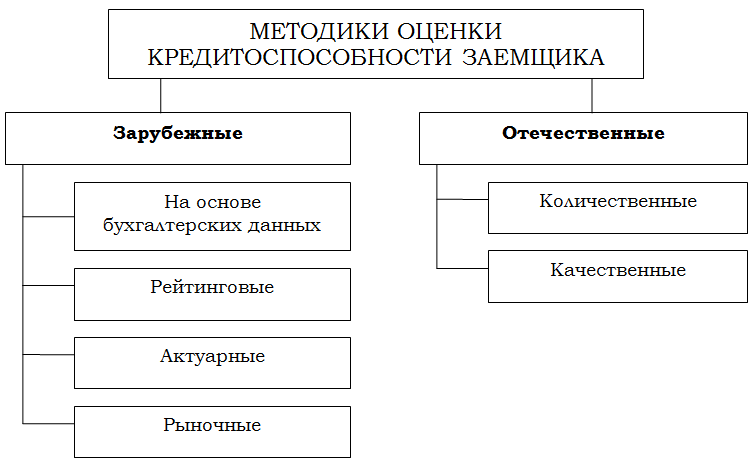
\includegraphics[width=0.9\textwidth]{media/image1.png} % Замените на реальный файл
    \caption{Классификация основных отечественных и зарубежных методик оценки кредитоспособности 
    предприятий}
    \label{fig:classification}
\end{figure}

Зарубежные методики оценки кредитоспособности предприятий можно ранжировать по четырем основным 
группам моделей, основанным на этих методиках [1].

К \textit{первой группе} относятся модели, базирующиеся исключительно на данных бухгалтерской отчетности. 
В таком случае устанавливается зависимость между вероятностью дефолта и финансовыми коэффициентами, 
рассчитанными на основе бухгалтерских данных. Данные модели отличаются достаточно высокой точностью 
прогнозов, однако они подвергаются критике за то, что чаще всего не принимают во внимание такие 
характеристики заемщика, как кредитная история, репутация, качество менеджмента и т.п. Примерами таких 
моделей являются модели Альтмана [6], Чессера [7], Фулмера [8], Олсона [9], Бивера [10], Таффлера и 
Тишоу [11], Спрингейта [12] и др.

\textit{Вторая группа} включает в себя модели, использующие как финансовую отчетность, так и 
дополнительные данные (рейтинговые модели), что позволяет всесторонне оценивать состояние заемщика, 
включая показатели развития отрасли экономики, к которой он принадлежит. В рейтинговых моделях [13, 14] 
преимущественно используется следующая информация:
\begin{itemize}
    \item оценка внешней среды контрагента (состояние отрасли, в которой контрагент осуществляет свою 
    деятельность, занимаемая доля на рынке, география операций и др.);
    \item оценка качества управления (опыт, компетентность, репутация и деловые качества руководителя);
    \item кредитная история (длительность взаимоотношений заемщика с кредитными организациями, 
    своевременность исполнения обязательств);
    \item характеристики кредитного продукта (срок, сумма, процентная ставка, комиссии, вид и сумма 
    обеспечения);
    \item анализ бухгалтерской отчетности и основных финансовых коэффициентов (рентабельность, 
    оборачиваемость, соотношение собственных и заемных средств, анализ денежных потоков).
\end{itemize}

В западных странах рейтинговые модели являются эталоном технологий управления кредитным риском [15]. 
Вместе с тем сам факт существования в каждой стране национальных моделей свидетельствует о том, что 
при их создании важнейшую роль играет страновая специфика. В связи с этим разработка рейтинговых моделей, 
учитывающих специфику отечественных экономических отношений, остается одной из актуальнейших задач 
управления кредитным риском в коммерческих банках Республики Беларусь.

В основе \textit{третьей группы} лежат математические (актуарные, эконометрические) модели оценки 
вероятности дефолта, которые рассчитываются рейтинговыми агентствами, классифицирующими предприятия и 
их долговые обязательства по вероятности дефолта путем присвоения им различных кредитных рейтингов [16]. 
Информационной основой подобных моделей выступает статистика дефолта по облигациям.

\textit{Четвертая группа} содержит модели, индикатором кредитного риска в которых является рыночная 
стоимость обращающихся на рынке облигаций, акций и кредитных производных инструментов, отражающая 
ожидания участников рынка в отношении возможности дефолта предприятия-эмитента [17]. Предполагается, 
что данная оценка должна быть более точной, чем основанная на математических моделях, поскольку рынок 
в каждый момент времени учитывает колоссальный объем поступающей информации макро- и микроэкономического, 
политического и психологического характера.

\subsection{Отечественная практика оценки кредитоспособности}

Каждый банк по-своему решает методологическую проблему оценки кредитоспособности заемщиков. Как отмечают 
многие отечественные эксперты в области банковского дела, применение иностранных моделей прогнозирования 
дефолта предприятий в отечественных условиях, как правило, не дает достаточно точных результатов. А 
вместе с тем разработка более точных моделей, базирующихся на собственном опыте, зачастую осложняется 
отсутствием необходимого количества надежных статистических данных. Чаще всего используются качественный 
и количественный методы анализа [1].

Как известно, основным критерием кредитоспособности выступает финансовое состояние заемщика, анализ 
которого проводится по следующим направлениям [18]:
\begin{itemize}
    \item финансовые результаты (прибыль, убыток);
    \item ликвидность (платежеспособность);
    \item рыночная позиция (деловая активность, конкурентоспособность, устойчивая динамика положения на 
    рынке);
    \item движение денежных потоков, прогноз на срок кредитования.
\end{itemize}

Корректирующими показателями оценки могут являться качественные факторы деятельности заемщика: 
положительная кредитная история; предоставление документов по первому требованию; качество управления, 
включая личностные характеристики и компетентность руководства предприятия-заемщика; деловая репутация; 
степень зависимости от государственных дотаций; общее состояние рынка по отрасли; общие позиции 
предприятия в конкурентной борьбе в его секторе или отрасли.

\textit{Качественные методы} оценки и прогнозирования вероятности дефолта имеют свои преимущества и 
недостатки [19]. С одной стороны, в отличие от количественных методов они позволяют подробно 
анализировать состояние организации, а не ориентируются на один критерий, который на практике может 
искажаться под воздействием различных обстоятельств (особенностей сферы деятельности организации, отрасли, 
страны, других факторов). С другой стороны, качественным методам в большей степени присуща субъективность, 
и их результат во многом зависит от квалификации и убеждений эксперта, проводящего анализ. Кроме этого, 
проведение качественного анализа требует значительных трудозатрат, а в некоторых случаях и наличия данных 
о деятельности компании, доступ к которым ограничен.

\textit{Количественные модели} основываются, как правило, на анализе некоторого набора финансовых 
коэффициентов, рассчитанных на основе данных финансовой отчетности предприятия, а также сравнения 
рассчитанных коэффициентов с эталонными значениями [18, 20].

Подводя итог, можно отметить, что обзор уже существующих подходов и методов оценки кредитоспособности 
нефинансовых предприятий демонстрирует актуальность разработки отечественных методик, которые учитывают 
особенности существующих экономических отношений, а также использующих комплексный подход. Наибольший 
интерес в данной задаче представляет разработка рейтинговых моделей, построенных с применением 
математико-статистического аппарата и оцененных по данным, собранным Национальным Банком по финансовым 
и нефинансовым организациям Республики Беларусь. Именно такие модели позволяют разрабатывать гибкие 
классификационные шкалы с произвольным числом градаций, использовать дополнительную актуальную информацию, 
а также учитывать особенности отдельных отраслей экономики.

\clearpage

% ==== 2 ИСПОЛЬЗУЕМЫЙ ПОДХОД ... ====
\section{ИСПОЛЬЗУЕМЫЙ ПОДХОД, МЕТОДЫ И АЛГОРИТМЫ ПОСТРОЕНИЯ СТАТИСТИЧЕСКИХ КРЕДИТНЫХ РЕЙТИНГОВ}

\subsection{Математическое описание модели данных}

Используется модель данных, представленная в [1].

В пространстве $R^{N}$ в моменты времени $t\ (t=1,\ldots,T)$ наблюдается $n$ объектов, которые 
относятся к одному из $K$ групп $G_{1},\ldots,G_{K}$. Для заданных условий $t,k$ объект $i$ 
(далее --- объект $(i,t,k)$) определяется случайным $N$-мерным вектором значений анализируемых финансовых 
показателей
\[
x_{i,t}^{(k)} \in R^{N}\ (i=1,\ldots,n,\ t=1,\ldots,T,\ k=1,\ldots,K)
\]
с вероятностной моделью, определяемой условной для заданных значений $(t,k)$ некоторой плотностью распределения $f^{(t,k)}(u),\ u \in R^{N}\ (t=1,\ldots,T,\ k=1,\ldots,K)$.

За период наблюдения $T$ получены выборки значений анализируемых показателей:
\begin{itemize}
    \item $X_{t}^{(k)} = \left\{ x_{i,t}^{(k)} \right\}\ (k=1,\ldots,K)$ --- выборка наблюдений в момент времени $t$ для объектов вида $G_{k}$,
    \item $X_{t} = \bigcup_{k=1}^{K} X_{t}^{(k)}$ --- выборка наблюдений в момент времени $t$ для всех объектов,
    \item $n_{t}^{(k)} = |X_{t}^{(k)}|,\ n_{t} = |X_{t}| = \sum_{k=1}^{K} n_{t}^{(k)}$ --- объемы соответствующих выборок.
\end{itemize}

По степени выраженности некоторого свойства $\nu \in S(L) = \{1,\ldots,L\}$ объекты делятся на $L$ классов $\Omega_{1},\ldots,\Omega_{L}$. Для заданных $t,k,i$ значение показателя $\nu$ обозначается $\nu_{i,t}^{(k)} \in S(L)$.

Таким образом, \textit{полная информация} об объекте $(i,t,k)$ определяется составным случайным вектором
\begin{equation}
z_{i,t}^{(k)} = \begin{pmatrix}
x_{i,t}^{(k)} \\
\nu_{i,t}^{(k)}
\end{pmatrix} \in R^{N} \times S(L)\ (i=1,\ldots,n_{t}^{(k)},\ t=1,\ldots,T).
\end{equation}

\textbf{Содержательная интерпретация модели.} В контексте рассматриваемой в рамках данного исследования задачи используется следующая содержательная интерпретация используемых выше понятий:
\begin{itemize}
    \item объекты --- это предприятия, относящиеся к одному из $K$ видов экономической деятельности (отраслей) $G_{1},\ldots,G_{K}$ и характеризуемые вектором значений финансовых показателей $x_{i,t}^{(k)}\ (i=1,\ldots,n_{k},\ t=1,\ldots,T,\ k=1,\ldots,K)$;
    \item $\Omega_{1},\ldots,\Omega_{L}$ --- классы кредитоспособности предприятий;
    \item $\nu_{i,t}^{(k)}$ --- неизвестный номер класса кредитоспособности предприятия $i$ из отрасли $k$ (далее --- предприятия $(i,k)$) в момент времени (квартал, год) $t\ (i=1,\ldots,n_{k},\ t=1,\ldots,T)$ [1].
\end{itemize}

\textit{Задача} статистической \textit{классификации} состоит в отнесении наблюдаемых объектов по наблюдениям $x_{i,t}^{(k)}$, удовлетворяющим рассматриваемой модели, к одному из классов $\Omega_{1},\ldots,\Omega_{L}$. Другими словами, имеет место задача статистической классификации объектов $(i,t,k)$, которая заключается в построении отображения
\[
d_{i,t}^{(k)} \equiv d(x_{i,t}^{(k)}): R^{N} \rightarrow S(L)\ (i=1,\ldots,n_{t}^{(k)},\ t=1,\ldots,T,\ k=1,\ldots,K).
\]

При упрощающем предположении о том, что в течение всего временного периода наблюдается одна и та же «сквозная» выборка объектов, можно положить, что
\[
n_{k} \equiv n_{t}^{(k)}\ \forall t=1,\ldots,T.
\]
Результатом решения сформулированной задачи исследования для всех видов объектов является $(n_{k} \times T)$-матрицы классификации объектов
\[
D^{(k)} = \left( d_{i,t}^{(k)} \right) = \begin{pmatrix}
d_{1,1}^{(k)} & \ldots & d_{1,T}^{(k)} \\
\vdots & \ddots & \vdots \\
d_{n_{k},1}^{(k)} & \cdots & d_{n_{k},T}^{(k)}
\end{pmatrix}\ (k=1,\ldots,K).
\]

Матрица классификации $D^{(k)}$ допускает представления по строкам и по столбцам, которые имеют содержательную экономическую интерпретацию
\[
D^{(k)} = \begin{pmatrix}
{d_{1}^{(k)}}' \\
\vdots \\
{d_{n_{k}}^{(k)}}'
\end{pmatrix},
\]
где
\[
{d_{i}^{(k)}}' = \left( d_{i1}^{(k)},\ldots,d_{iT}^{(k)} \right) \in S^{T}(L)\ (i=1,\ldots,n_{k})
\]
--- вектор классификации, отражающий динамику изменения класса кредитоспособности (рейтинга) $i$-го предприятия из $k$-ой отрасли;

\[
D^{(k)} = \left( \delta_{1}^{(k)},\ldots,\delta_{T}^{(k)} \right),
\]
где
\[
\delta_{t}^{(k)} = \left( \delta_{1,t}^{(k)},\ldots,\delta_{n_{k},t}^{(k)} \right) \in S^{n_{k}}(L)\ (t=1,\ldots,T)
\]
--- вектор классификации объектов $k$-го вида для момента времени $t$.

При известных векторах $d_{i}^{(k)}\ (i=1,\ldots,n_{k}),\ \delta_{t}^{(k)}\ (t=1,\ldots,T)$ могут быть рассчитаны такие обобщенные показатели кредитоспособности на микро- и макроуровне как:
\begin{itemize}
    \item средний рейтинг предприятия за рассматриваемый период наблюдения:
    \[
    \overline{d}_{i}^{(k)} = \frac{1}{T}\sum_{t=1}^{T} d_{it}^{(k)} \in [1,L]\ (i=1,\ldots,n_{k});
    \]
    \item средний отраслевой рейтинг в фиксированный момент времени $t$:
    \[
    \overline{\delta}_{t}^{(k)} = \frac{1}{n_{k}}\sum_{i=1}^{n_{k}} \delta_{it}^{(k)} \in [1,L]\ (t=1,\ldots,T).
    \]
\end{itemize}
Временной ряд $\overline{\delta}_{t}^{(k)}\ (t=1,\ldots,T)$ описывает динамику изменения отраслевого рейтинга для $k$-ой отрасли за рассматриваемый период наблюдения.

\subsection{Этапы построения статистических кредитных рейтингов}

\subsubsection{Общее описание схемы используемого подхода}

В работе реализуется подход к построению статистических кредитных рейтингов, представленный в [1]:
\begin{enumerate}
    \item Предварительный статистический анализ данных;
    \item Исследование статистической зависимости на основе 
    корреляционного анализа;
    \item Формирование классификационных признаков (интегрального 
    показателя) на основе метода главных компонент;
    \item Построение кластеров, разделяющих предприятия по кредитным 
    рейтингам при помощи алгоритма K-средних;
    \item Построение кластеров, разделяющих предприятия по кредитным 
    рейтингам при помощи алгоритма иерархического агломеративного 
    кластерного анализа данных.
    \item Классификация кредитоспособности на основе мультиномиальной 
    логистической регрессии.
\end{enumerate}

\subsubsection{Выявление аномалий при помощи алгоритма Isolation Forest и их цензурирование}

Для выявления аномальных наблюдений был использован алгоритм машинного обучения \textit{Isolation Forest}.

Алгоритм \textit{Isolation Forest} состоит из двух основных этапов: этап обучения 
(построение ансамбля деревьев изоляции) и этап оценивания (вычисление показателя аномальности для 
каждого наблюдения).

\textbf{Этап 1. Обучение ансамбля деревьев изоляции.}

Входные параметры: набор данных $X$ размером $N$ наблюдений, количество деревьев в ансамбле $T$, размер 
подвыборки для одного дерева $\psi$ (в рассматриваемой задаче в качестве $\psi$ взято значение $256$).

\begin{itemize}
\item[Шаг 1.] Инициализация пустого леса Forest.
\item[Шаг 2.] Для каждого дерева с индексом $t$ от 1 до $T$:
\begin{itemize}
    \item[Шаг 2.1.] Случайным образом без возвращения отобрать подвыборку $X'$ размером $\psi$ из исходного 
    набора данных $X$.
    \item[Шаг 2.2.] Построить дерево изоляции $\text{iTree}(X', 0)$, где второй аргумент обозначает текущую 
    глубину дерева. Процедура построения $\text{iTree}(\text{node\_data}, \text{current\_depth})$ выполняется 
    рекурсивно:
    \begin{itemize}
        \item[Шаг 2.2.1.] Проверить условие остановки: если current\_depth достиг предельной глубины 
        (которая в среднем ограничена значением $\lceil \log_{2}(\psi) \rceil$) или количество наблюдений 
        в узле меньше или равно единице, то создать листовой узел и вернуть его.
        \item[Шаг 2.2.2.] В противном случае случайным образом выбрать один из признаков $q$ из всего 
        множества признаков данных.
        \item[Шаг 2.2.3.] Случайным образом выбрать точку разделения $p$ из интервала значений признака 
        $q$, определяемого минимальным и максимальным значением этого признака в текущей подвыборке 
        node\_data.
        \item[Шаг 2.2.4.] Разделить подвыборку node\_data на две части: левую часть $L$, содержащую 
        наблюдения, у которых значение признака $q$ меньше $p$, и правую часть $R$, содержащую наблюдения, 
        у которых значение признака $q$ больше либо равно $p$.
        \item[Шаг 2.2.5.] Рекурсивно вызвать процедуру построения для левого и правого подмножеств: 
        $\text{iTree}(L, \text{current\_depth} + 1)$ и $\text{iTree}(R, \text{current\_depth} + 1)$.
    \end{itemize}
    \item[Шаг 2.3.] Добавить построенное дерево в ансамбль Forest.
\end{itemize}
\item[Шаг 3.] Вернуть построенный ансамбль Forest.
\end{itemize}

Следующим этапом обработки аномальных наблюдений является цензурирование выборки \cite{23}, то есть 
замена аномально больших и малых значений коэффициентов на экономически и статистически
обоснованные максимальные и минимальные пороговые значения $K_{min}, K_{max}$. Значения рассматриваемых 
показателей, не попадающие в заданный диапазон, подвергаются цензурированию. Диапазон выбирается на основе 
значений показателей, соответствующих наблюдениям, классифицированным как нормальные (неаномальные). Для 
каждого финансового коэффициента $X^{(j)}$ по подмножеству $\mathcal{N}$ неаномальных объектов вычисляются 
минимальное и максимальное значения:
\[
K_{\min}^{(j)} = \min_{i \in \mathcal{N}} X_i^{(j)}, \qquad 
K_{\max}^{(j)} = \max_{i \in \mathcal{N}} X_i^{(j)},
\]
где $i$ — индекс наблюдения, $j$ — индекс признака. Полученные величины принимаются в качестве пороговых 
значений, ограничивающих допустимую область вариации признака.

Для каждого наблюдения $i$, отнесённого к аномальным ($i \in \mathcal{A}$), значения коэффициентов, 
выходящие за пределы интервала $[K_{\min}^{(j)}, K_{\max}^{(j)}]$, подвергаются цензурированию:
\[
\tilde{X}_i^{(j)} = 
\begin{cases}
K_{\min}^{(j)}, & \text{если } X_i^{(j)} < K_{\min}^{(j)}, \\[4pt]
K_{\max}^{(j)}, & \text{если } X_i^{(j)} > K_{\max}^{(j)}, \\[4pt]
X_i^{(j)}, & \text{иначе}.
\end{cases}
\]

Такой подход \cite{23} позволяет зафиксировать экономически и статистически обоснованные границы 
допустимых значений, исключающие влияние выбросов, и при этом сохранить все единицы совокупности в анализе, 
не прибегая к удалению наблюдений.

\subsubsection{Предварительный статистический анализ данных}

В рамках предварительного анализа данных была осуществлена следующая обработка данных:
\begin{enumerate}
    \item \textit{Выявление и исключение аномальных наблюдений}: для выявления аномальных наблюдений был 
    использован алгоритм машинного обучения Elliptic Envelope. Он строит робастную оценку ковариационной 
    матрицы, ограничивает центр распределения эллипсом, игнорируя при этом наблюдения, которые находятся 
    снаружи.
    \item \textit{Нормировка данных} (приведение всех коэффициентов к размерности $[0,1]$)
\end{enumerate}
Для возможности более удобной интерпретации результатов производится приведение значений всех рассчитанных 
финансовых коэффициентов к шкале $[0,1]$. При этом более высокие значения показателей соответствуют 
предприятиям с более высокой степенью кредитоспособности. С этой целью используются следующие формулы:
\[
K^{norm} = \frac{K - K_{\min}}{K_{\max} - K_{\min}} \quad \text{или} \quad K^{norm} = \frac{K_{\max} - K}
{K_{\max} - K_{\min}}
\]
для случаев прямой и обратной зависимости кредитоспособности от рассматриваемого показателя.

\subsubsection{Исследование статистической зависимости финансовых коэффициентов на основе корреляционного 
анализа}

Для обнаружения и оценки «парной» зависимости между двумя компонентами $X_{i}, X_{j}\ (i \neq j)$ 
используется коэффициент корреляции \cite{2}:
\begin{equation}
\rho_{ij} = \frac{\sigma_{ij}}{\sqrt{\sigma_{ii}\sigma_{jj}}} \in [-1,1],
\end{equation}
являющийся мерой линейной статистической зависимости между случайными величинами $X_{i}$ и $X_{j}$.

Асимптотически несмещённой и состоятельной оценкой $\rho_{ij}$ по выборке $X$ является \textit{выборочный 
коэффициент корреляции} [2]:
\begin{equation}
r_{ij} = \frac{\sum_{t=1}^{n} (x_{ti} - \overline{x_{i}})(x_{tj} - \overline{x_{j}})}{\sqrt{\sum_{t=1}^{n} 
(x_{ti} - \overline{x_{i}})^{2} \cdot \sum_{t=1}^{n} (x_{tj} - \overline{x_{j}})^{2}}} \in [-1,+1],
\end{equation}
где $\overline{x} = (\overline{x_{i}}) = \frac{1}{n}\sum_{t=1}^{n} z_{t}$ --- вектор-столбец выборочных 
средних.

\textbf{Этап 2. Вычисление оценки аномальности для наблюдения $x$.}

Входные данные: наблюдение $x$, ансамбль Forest из $T$ деревьев, размер подвыборки $\psi$.

Шаг 1. Для каждого дерева $t$ в ансамбле определить длину пути $h_{t}(x)$, пройденного наблюдением $x$ от корня дерева до листового узла. Длиной пути считается количество ребер (разбиений), которое потребовалось для изоляции наблюдения. Если наблюдение попадает в узел, который не является листовым, но был создан из-за ограничения по глубине, к текущей глубине добавляется поправка, равная ожидаемой длине пути для неудачного поиска в бинарном дереве поиска для количества элементов в этом узле.\\
Шаг 2. Вычислить среднюю длину пути $E(h(x))$ как среднее арифметическое значений $h_{t}(x)$ по всем $T$ деревьям.\\
Шаг 3. Вычислить оценку аномальности $s(x, \psi)$ по формуле:
\[
s(x, \psi) = 2^{ -E(h(x)) / c(\psi) },
\]
где $c(\psi)$ --- нормировочная константа, равная средней длине пути неудачного поиска в бинарном дереве поиска для $\psi$ элементов. Она вычисляется как:
\begin{align*}
c(\psi) &= 2 \cdot H(\psi - 1) - \frac{2(\psi - 1)}{\psi} \quad \text{при } \psi > 2,\\
c(\psi) &= 1 \quad \text{при } \psi = 2,\\
c(\psi) &= 0 \quad \text{при } \psi < 2.
\end{align*}
Здесь $H(i)$ --- $i$-ое гармоническое число, которое может быть аппроксимировано как $H(i) \approx \ln(i) + 0.5772156649$ (константа Эйлера-Маскерони).

Шаг 4. Интерпретация полученной оценки: если $s(x, \psi)$ близко к 1, то наблюдение с высокой вероятностью является аномалией; если $s(x, \psi)$ значительно меньше 0.5, то наблюдение, вероятно, является нормальным; если для всех наблюдений выборки $s(x, \psi) \approx 0.5$, то весь набор данных, по-видимому, не содержит выраженных аномалий.

\subsubsection{Формирование классификационных признаков по методу главных компонент}

Практическое применение метода главных компонент (МГК) предполагает выполнение следующих шагов [1]:

1. Преобразование исходных данных. Переход от исходной матрицы данных $X = (x_{ij})\ (i=1,\ldots,n,\ j=1,\ldots,N)$ объема $n$ к матрице $Z = (z_{ij})\ (i=1,\ldots,n,\ j=1,\ldots,N)$ \textit{нормированных признаков} по формулам:
\begin{equation}
\begin{gathered}
z_{ij} = \frac{x_{ij} - \overline{x}_{j}}{s_{j}}\ (i=1,\ldots,n,\ j=1,\ldots,N),\quad
\overline{x}_{j} = \frac{1}{n}\sum_{i=1}^{n} x_{ij},\quad \\
s_{j} = \sqrt{\frac{1}{n-1}\sum_{i=1}^{n} (x_{ij} - \overline{x}_{j})^{2}}.
\end{gathered}
\end{equation}

2. Вычисление матрицы парных корреляций для нормированных признаков
\begin{equation}
R = \frac{1}{n} Z' Z = (\rho_{ij})\ (i,j=1,\ldots,N).
\end{equation}

3. Вычисление матриц собственных векторов и собственных значений для корреляционной матрицы $R$:
\begin{itemize}
    \item матрицы \textit{собственных значений} $\Lambda = \operatorname{diag}\{\lambda_{i}\}\ (i=1,\ldots,N)$;
    \item матрицы \textit{ортонормированных собственных векторов} $\Phi = (\phi_{1}|\ldots|\phi_{N})$,
\end{itemize}
в результате решения задачи:
\begin{equation}
\Phi \Sigma \Phi' = \Lambda \Phi,\quad \Phi \Phi' = I_{N}.
\end{equation}

4. Вычисление матрицы факторного отображения $A = (a_{ij}) = \Phi \Lambda^{1/2}$, используемой для вычисления матрицы ортонормированных признаков на основе исходных признаков (вектор-столбцов) матрицы $Z = (z_{ij})\ (i=1,\ldots,n,\ j=1,\ldots,N)$.

Из свойства $A'A = \Lambda$ следует:
\begin{equation}
\sum_{i=1}^{n} a_{il}^{2} = \lambda_{l}.
\end{equation}

5. Вычисление матрицы ортонормированных признаков
\begin{equation}
F = (f_{1}|f_{2}|\ldots|f_{N}),\quad f_{k} = (f_{1k},f_{2k},\ldots,f_{nk})'\ (k=1,\ldots,N)
\end{equation}
по одной из формул:
\begin{align}
F &= A^{-1} Z,\\
F &= \Lambda^{-1/2} \Phi' Z'\ (k=1,\ldots,K,\ i=1,\ldots,n).
\end{align}

6. Выбор $K < N$ главных компонент $F = (f_{1}|f_{2}|\ldots|f_{K})\ (k=1,\ldots,K)$, соответствующих доминирующим собственным векторам, для которых $\lambda_{1} \geq \lambda_{2} \geq \ldots \geq \lambda_{K} > 1$, соответствующим собственным значениям большим 1.

7. Определение оптимального числа главных компонент на основе вклада компонент в общую дисперсию, объясняющих заданную долю общей дисперсии. Доля каждой главной компоненты равна собственному значению для соответствующего собственного вектора.

8. Вращение факторов с целью оптимизации значений факторных нагрузок $a_{ik}\ (i=1,\ldots,n,\ k=1,\ldots,K)$ и повышение интерпретируемости главных компонент.

Проблема интерпретации главных компонент, которая решается на основе анализа тесноты связи (корреляции) между главными компонентами и исходными переменными, определяемой факторными нагрузками. Для большей наглядности интерпретации используются дополнительные линейные преобразования вектора главных компонент, называемые вращениями (методы Варимакс, Квартимакс и др.). Указанные действия комментируются далее при проведении статистического анализа реальных данных.

9. Вычисление значений интегрального (сводного) показателя по формуле:
\begin{equation}
I_{i} = \delta_{1} f_{1i} + \delta_{2} f_{2i} + \ldots + \delta_{K} f_{Ki},\ i=1,\ldots,n,
\end{equation}
где весовой коэффициент $\delta_{k}$ выражает относительный вклад $k$-й $(k=1,\ldots,K)$ главной компоненты в общую дисперсию случайной векторной переменной $Z$ и вычисляется по формуле
\begin{equation}
\delta_{k} = \frac{\lambda_{k}}{\sum_{j=1}^{N} \lambda_{j}},\ k=1,\ldots,K.
\end{equation}

Переменные $f_{ki}$ и $I_{i}$ по построению центрированы относительно нуля, что является удобным при трактовке результатов в контексте рассматриваемой задачи: чем больше нуля интегральный показатель платежеспособности (кредитоспособности) предприятия, тем выше его уровень платежеспособности (кредитоспособности) и соответственно, чем меньше его значение, тем ниже уровень платежеспособности (кредитоспособности) предприятия.

Таким образом, интегральный показатель платежеспособности (кредитоспособности) позволяет классифицировать (ранжировать) все предприятия по уровню платежеспособности (кредитоспособности). Для этого должны быть определены интервалы значений интегрального показателя, соответствующие заданному числу классов. Результаты кластерного анализа могут использоваться для определения указанных границ.

\subsubsection{Построение статистических кредитных рейтингов на основе кластерного анализа в пространстве главных компонент}

Если вектор классификации $d = (d_{i}) \in S^{n}(L)$ для обучающей выборки не известен, то это существенно ограничивает класс возможных статистических алгоритмов для классификации заемщиков на основе доступной информации в виде векторов значений их финансовых показателей $x = (x_{1},\ldots,x_{N})' \in R^{N}$. Практически остается две основные возможности:
\begin{enumerate}
    \item использование алгоритмов кластерного анализа (в непараметрическом случае) и алгоритмов расщепления смесей распределения (в параметрическом случае) [4];
    \item классификация на основе интегрального показателя (индикатора), для построения которого обычно используются методы факторного анализа [3].
\end{enumerate}

\textbf{Использование метода K-средних}

Данный алгоритм основывается на предположении о взаимной компактности «кластеров», образованных из наблюдений одного класса. В соответствии с алгоритмом K-средних, для классификации наблюдения $x = (x_{1},\ldots,x_{N})' \in \mathbb{R}^{N}$ используется решающее правило [1]:
\begin{equation}
d = d(x,X) = \underset{l \in S(L)}{\operatorname{argmin}} \left| x - \hat{\mu}_{l} \right|,\ X \in \mathbb{R}^{n \times N},
\end{equation}
где центры кластеров $\{\hat{\mu}_{l}\}$ зависят от классифицируемой выборки $X \in \mathbb{R}^{nN}$ и определяются итерационным образом. Объект может быть отнесен только к одному из кластеров. Такой тип кластеризации называется жёсткой кластеризацией. Обозначение $|x - \hat{\mu}_{l}|$ означает расстояние между двумя точками с координатами $x,\hat{\mu}_{l}$ в пространстве $\mathbb{R}^{N}$.

Таким образом, правило (2.12) имеет простую интерпретацию: наблюдение $x = (x_{1},\ldots,x_{N})' \in \mathbb{R}^{N}$ относится к тому классу, расстояние до центра которого минимально [2]. Алгоритмы указанного типа просты в реализации и не имеют технических требований к объему выборки. В то же время существует проблема интерпретации получаемых разбиений выборки на кластеры, поскольку нумерация кластеров осуществляется в процессе работы алгоритма случайным образом. Следовательно, возникает необходимость перенумерации кластеров в соответствии со степенью выраженности оцениваемого качества классифицируемых объектов, которое не имеет однозначной интерпретации [1].

На нулевом шаге итерационного процесса выбираются начальные центры кластеров. На каждой последующей итерации происходит вычисление вектора решений по формуле (2.12) и уточняются центры кластеров. Точкой останова итерационного процесса является равенство векторов решений этой и следующей итерации [2].

\textbf{Использование иерархического агломеративного метода}

Алгоритм иерархического агломеративного кластерного (ИАК) анализа данных применяется, когда число классов объектов не известно. В результате работы итерационного алгоритма ИАК на каждой итерации получаются разбиения исходной выборки на определенное число кластеров. С каждой новой итерации число кластеров сокращается от $n$ (на начальной итерации число кластеров полагается равным объему выборки: каждое наблюдение считается отдельным кластером) до определенного числа $n'\ (1 \leq n' \leq n)$ кластеров, имеющих наилучшую содержательную интерпретацию и статистические свойства. Этот метод основан на отыскании и слиянии наиболее близких кластеров; он реализуется с помощью следующей итерационной процедуры.

\textbf{Описание процедуры классификации.} [2] Обозначим $t \in \{0,1,\ldots,n-1\}$ текущий номер итерации; $\hat{W}_{1}^{t},\ldots,\hat{W}_{L_{t}}^{t}$ --- набор кластеров на $t$-й итерации, $L_{t} \in \{1,\ldots,n\}$ --- число кластеров на $t$-й итерации.

В момент $t$ задаётся $n$ одноэлементных кластеров. Пусть произошла итерация $t$ и получен набор $L_{t}$ кластеров: $\hat{W}_{1}^{t},\ldots,\hat{W}_{L_{t}}^{t}$. Найдём пару $(i^{*},j^{*})\ (1 \leq i < j \leq L_{t})$ наиболее близких кластеров:
\begin{equation}
\rho\left( \hat{W}_{i}^{t},\hat{W}_{j}^{t} \right) \rightarrow \min_{1 \leq i < j \leq L_{t}},
\end{equation}
где в качестве $\rho$ применима одна из следующих метрик:
\begin{align}
\rho_{1}\left( \hat{W}_{i}^{t},\hat{W}_{j}^{t} \right) &= \min_{x \in \hat{W}_{i}^{t},\ y \in \hat{W}_{j}^{t}} |x - y|,\\
\rho_{2}\left( \hat{W}_{i}^{t},\hat{W}_{j}^{t} \right) &= \max_{x \in \hat{W}_{i}^{t},\ y \in \hat{W}_{j}^{t}} |x - y|,\\
\rho_{3}\left( \hat{W}_{i}^{t},\hat{W}_{j}^{t} \right) &= \frac{1}{|\hat{W}_{i}^{t}| |\hat{W}_{j}^{t}|} \sum_{x \in \hat{W}_{i}^{t}} \sum_{y \in \hat{W}_{j}^{t}} |x - y|.
\end{align}

После этого кластеры с минимальной метрикой между ними объединяются в один, и $L_{t+1} = L_{t} - 1$. Итерационный процесс продолжается, пока $L_{t} > L$. Иногда процесс продолжается до $L_{t+1} = 1$.

\subsubsection{Классификация кредитоспособности на основе мультиномиальной 
    логистической регрессии.}

Для классификации 

\clearpage

% ==== 3 РЕЗУЛЬТАТЫ ПОСТРОЕНИЯ ... ====
\section{РЕЗУЛЬТАТЫ ПОСТРОЕНИЯ СТАТИСТИЧЕСКИХ КРЕДИТНЫХ РЕЙТИНГОВ НА ОСНОВЕ ИСПОЛЬЗУЕМОГО ПОДХОДА}

\subsection{Описание данных финансовой отчётности}

Анализируемая выборка представляет собой статистические данные по нефинансовым предприятиям. Источником информации является бухгалтерская отчетность субъектов хозяйствования, представленная на отчетную дату (бухгалтерский баланс, отчет о прибылях и убытках). С точки зрения отчетного периода имеются 2 типа данных: годовые данные (информация представляется за отчетный год) и квартальные данные (информация представляется за отчетные периоды: 3 месяца, 6 месяцев, 9 месяцев, 12 месяцев). С целью сокращения исходного пространства признаков и перехода к безразмерным показателям формируется множество финансовых коэффициентов. Для наиболее полного и многостороннего анализа финансового состояния предприятий были отобраны коэффициенты из 5 групп, характеризующие различные стороны финансово-хозяйственной деятельности предприятий. Далее приводится список финансовых коэффициентов, формулы их расчета даны в Приложении.

\begin{enumerate}[label=\Roman*.]
    \item \textit{Показатели ликвидности}
    \begin{itemize}
        \item K1 -- коэффициент текущей ликвидности;
        \item K2 -- коэффициент абсолютной ликвидности;
        \item K3 -- коэффициент ликвидности средств в обращении (коэффициент быстрой (срочной) ликвидности);
    \end{itemize}
    
    \item \textit{Коэффициенты финансовой устойчивости}
    \begin{itemize}
        \item K4 -- коэффициент обеспеченности собственными оборотными средствами;
        \item K5 -- коэффициент обеспеченности финансовых обязательств активами;
        \item K6 -- качество дебиторской задолженности;
        \item K7 -- качество кредиторской задолженности;
        \item K8 -- коэффициент финансовой независимости;
        \item K9 -- коэффициент финансирования;
        \item K10 -- коэффициент мобильности средств;
    \end{itemize}
    
    \item \textit{Коэффициенты динамики развития}
    \begin{itemize}
        \item K11 -- темпы роста выручки;
        \item K12 -- рост капитала;
    \end{itemize}
    
    \item \textit{Коэффициенты деловой активности}
    \begin{itemize}
        \item K13 -- коэффициент оборачиваемости активов;
        \item K14 -- коэффициент оборачиваемости кредиторской задолженности;
        \item K15 -- коэффициент оборачиваемости дебиторской задолженности;
        \item K16 -- коэффициент соотношения длительности периодов оборачиваемости дебиторской задолженности и кредиторской задолженности;
        \item K17 -- коэффициент оборачиваемости товарных запасов;
    \end{itemize}
    
    \item \textit{Коэффициенты рентабельности (эффективности деятельности)}
    \begin{itemize}
        \item K18 -- коэффициент рентабельности продукции;
        \item K19 -- коэффициент рентабельности активов;
        \item K20 -- коэффициент рентабельности капитала.
    \end{itemize}
\end{enumerate}

\subsection{Результаты применения корреляционного анализа}

В таблице 3.1 приведены коэффициенты парной корреляции для коэффициентов K1--K10 (приведены значения верхнего треугольника, так как матрица симметрична). Большинство анализируемых коэффициентов демонстрирует наличие статистически значимой взаимосвязи с остальными показателями. Наиболее сильная взаимосвязь наблюдается между коэффициентами K5 и K8.

\begin{table}[H]
    \centering
    \caption{Матрица парных корреляций между коэффициентами K1--K10}
    \label{tab:corr}
    \small
    \begin{tabular}{c|cccccccccc}
        \toprule
        & K1 & K2 & K3 & K4 & K5 & K6 & K7 & K8 & K9 & K10 \\
        \midrule
        K1  & 1.0  & 0.66 & 0.85 & 0.51 & -0.45 & -0.1  & -0.25 & 0.45 & 0.49 & 0.09 \\
        K2  & 0.66 & 1.0  & 0.76 & 0.36 & -0.34 & -0.12 & -0.24 & 0.34 & 0.33 & 0.06 \\
        K3  & 0.85 & 0.76 & 1.0  & 0.43 & -0.36 & -0.09 & -0.23 & 0.36 & 0.42 & 0.11 \\
        K4  & 0.51 & 0.36 & 0.43 & 1.0  & -0.58 & -0.07 & -0.25 & 0.58 & 0.29 & 0.22 \\
        K5  & -0.45& -0.34& -0.36& -0.58& 1.0   & 0.02  & 0.14  & -1.0  & -0.59& 0.45 \\
        K6  & -0.1 & -0.12& -0.09& -0.07& 0.02  & 1.0   & 0.39  & -0.01 & -0.01& -0.08\\
        K7  & -0.25& -0.24& -0.23& -0.25& 0.14  & 0.39  & 1.0   & -0.14 & -0.13& -0.08\\
        K8  & 0.45 & 0.34 & 0.36 & 0.58 & -1.0  & -0.01 & -0.14 & 1.0   & 0.59 & -0.45\\
        K9  & 0.49 & 0.33 & 0.42 & 0.29 & -0.59 & -0.01 & -0.13 & 0.59  & 1.0  & -0.33\\
        K10 & 0.09 & 0.06 & 0.11 & 0.22 & 0.45  & -0.08 & -0.08 & -0.45 & -0.33& 1.0 \\
        \bottomrule
    \end{tabular}
\end{table}

В соответствии с полученными результатами из дальнейшего анализа целесообразно исключить коэффициент K8, так как для него существует корреляция близкая к $-1$ с коэффициентом K5.

\subsection{Результаты формирования классификационных признаков с помощью метода главных компонент}

Для оценки целесообразности применения метода главных компонент воспользуемся \textit{критерием сферичности Бартлетта} [21] и \textit{статистикой Кайзера--Мейера--Олкина} [22].

В соответствии с таблицей 3.2, нулевая гипотеза о том, что корреляционная матрица является единичной, отклоняется критерием сферичности Бартлетта. Приближенное значение статистики равно 28628,405, она является значимой на уровне 0,05. Значение статистики КМО, равное 0,780, свидетельствует о приемлемом качестве выборки для применения факторного анализа при пороговом значении в 0,6.

\begin{table}[H]
    \centering
    \caption{Анализ пригодности выборочной корреляционной матрицы}
    \label{tab:kmo}
    \begin{tabular}{llr}
        \toprule
        \multicolumn{2}{l}{Статистика Кайзера--Мейера--Олкина} & 0,703 \\
        \midrule
        \multirow{2}{*}{Критерий сферичности Бартлетта} & Статистика $\chi^{2}$ & 28385,439 \\
        & $p$-значение & 0,000 \\
        \bottomrule
    \end{tabular}
\end{table}

Согласно таблице 3.3, в совокупности выделенные факторы объясняют 61,357\% дисперсии исходных показателей, в частности, первый фактор до вращения объясняет 25,891\% дисперсии, второй --- 12,713\%, третий --- 8,391\%, четвертый --- 6,16\%, пятый --- 4,547\% и шестой --- 3,653\%. Вращение факторов приводит к более равномерному распределению объясненной дисперсии между факторами и к увеличению удельного веса каждого из них. Таким образом, на долю первого фактора после вращения приходится 14,45\% объясненной дисперсии, второго --- 11,45\%, третьего --- 9,908\%, четвертого --- 9,688\%, пятого --- 8,513\%, шестого --- 7,347\%.

\begin{table}[H]
    \centering
    \caption{Собственные значения и объяснённая дисперсия}
    \label{tab:eigen}
    \small
    \begin{tabular}{c|ccc|ccc}
        \toprule
        № & \multicolumn{3}{c|}{Начальные факторы до вращения} & \multicolumn{3}{c}{Факторы после вращения} \\
        фактора & Собств. знач. & Доля дисп. & Кумул. доля & Собств. знач. & Доля дисп. & Кумул. доля \\
        \midrule
        1 & 5.1988654 & 0.2589156 & 0.25891566 & 2.7455760 & 0.144504 & 0.144504 \\
        2 & 2.6982210 & 0.1271296 & 0.38604526 & 2.1755476 & 0.1145025 & 0.25900651 \\
        3 & 1.8471020 & 0.0839117 & 0.46995702 & 1.8825394 & 0.0990810 & 0.35808754 \\
        4 & 1.5908083 & 0.0616097 & 0.53156681 & 1.8407216 & 0.0968800 & 0.45496762 \\
        5 & 1.2196680 & 0.0454738 & 0.5770407  & 1.6175588 & 0.0851346 & 0.5401023 \\
        6 & 1.1126349 & 0.0365342 & 0.6135749  & 1.3959795 & 0.0734726 & 0.6135749 \\
        \bottomrule
    \end{tabular}
\end{table}

Для интерпретации факторов используется анализ факторных нагрузок до и после вращения факторов, приведенные для используемой выборки в таблицах 3.4 и 3.5 соответственно.

Вращение факторов позволяет достичь более простой структуры факторных нагрузок для исходных переменных, что может несколько упростить интерпретацию полученных факторов.

После применения процедуры вращения с первой главной компонентой наиболее тесно коррелируют показатели ликвидности, со второй --- коэффициенты деловой активности, с третьей --- коэффициент обеспеченности финансовых обязательств активами и коэффициент мобильности средств, с четвёртой --- коэффициент обеспеченности собственными оборотными средствами и коэффициенты рентабельности, с пятой --- коэффициенты динамики развития и с шестой --- коэффициент оборачиваемости дебиторской задолженности и коэффициент соотношения длительности периодов оборачиваемости.

% Таблицы факторных нагрузок опущены для краткости, но могут быть добавлены аналогично

\subsection{Результаты классификации, полученные с помощью алгоритма K-средних}

Для классификации рассматриваемой выборки предприятий используется алгоритм K-средних в пространстве главных компонент. Количество кластеров задавалось равным четырём.

В таблице 3.6 приведены координаты центров кластеров в пространстве главных компонент.

\begin{table}[H]
    \centering
    \caption{Координаты центров кластеров, полученных методом K-средних}
    \label{tab:kmeans_centers}
    \begin{tabular}{c|cccccc}
        \toprule
        Кластер & PC1 & PC2 & PC3 & PC4 & PC5 & PC6 \\
        \midrule
        1 & 2.4802 & 0.2177 & -0.2769 & 0.0211 & 0.0347 & -0.2379 \\
        2 & -0.2965 & -0.4605 & -0.7767 & 0.1989 & -0.2963 & 0.0117 \\
        3 & -0.2374 & -0.0579 & 0.787 & -0.8715 & -0.0156 & -0.2859 \\
        4 & -0.1667 & 0.6644 & 0.2972 & 0.737 & 0.4365 & 0.408 \\
        \bottomrule
    \end{tabular}
\end{table}

В таблице 3.7 предоставлено, каким образом переопределялась нумерация кластеров в зависимости от значений интегрального показателя.

\begin{table}[H]
    \centering
    \caption{Переопределение номеров кластеров}
    \label{tab:recode}
    \begin{tabular}{cc}
        \toprule
        Номер кластера (алгоритм) & Номер кластера (интегральный показатель) \\
        \midrule
        4 & 2 \\
        3 & 3 \\
        2 & 4 \\
        1 & 1 \\
        \bottomrule
    \end{tabular}
\end{table}

В таблице 3.8 представлено число наблюдений в каждом кластере с изменённой нумерацией.

\begin{table}[H]
    \centering
    \caption{Количество наблюдений в каждом кластере}
    \label{tab:counts}
    \begin{tabular}{ccc}
        \toprule
        Номер кластера & Количество наблюдений & Относительная частота \\
        \midrule
        1 & 215 & 0,08866 \\
        2 & 605 & 0,2495 \\
        3 & 720 & 0,2969 \\
        4 & 885 & 0,3649 \\
        \bottomrule
    \end{tabular}
\end{table}

В таблице 3.9 представлена описательная статистика для интегрального показателя в разрезе выделенных кластеров.

\begin{table}[H]
    \centering
    \caption{Описательная статистика для интегральных показателей}
    \label{tab:desc_kmeans}
    \begin{tabular}{c|ccccc}
        \toprule
        Номер кластера & Среднее & Медиана & Минимум & Максимум & Станд. откл. \\
        \midrule
        1 & 0.3434 & 0.3275 & -0.31 & 1.19 & 0.2546 \\
        2 & 0.22   & 0.1893 & -0.06 & 0.94 & 0.1789 \\
        3 & -0.0697& -0.0692& -0.68 & 0.5  & 0.1376 \\
        4 & -0.1776& -0.1799& -0.64 & 0.16 & 0.1301 \\
        \bottomrule
    \end{tabular}
\end{table}

\subsection{Результаты классификации, полученные с помощью алгоритма иерархического кластерного анализа}

В качестве второго способа классификации предприятий по кредитным рейтингам применяется метод агломеративного иерархического кластерного анализа.

На рисунке 3.1 представлена дендрограмма для метода Ward с метрикой Euclidean.

\begin{figure}[H]
    \centering
    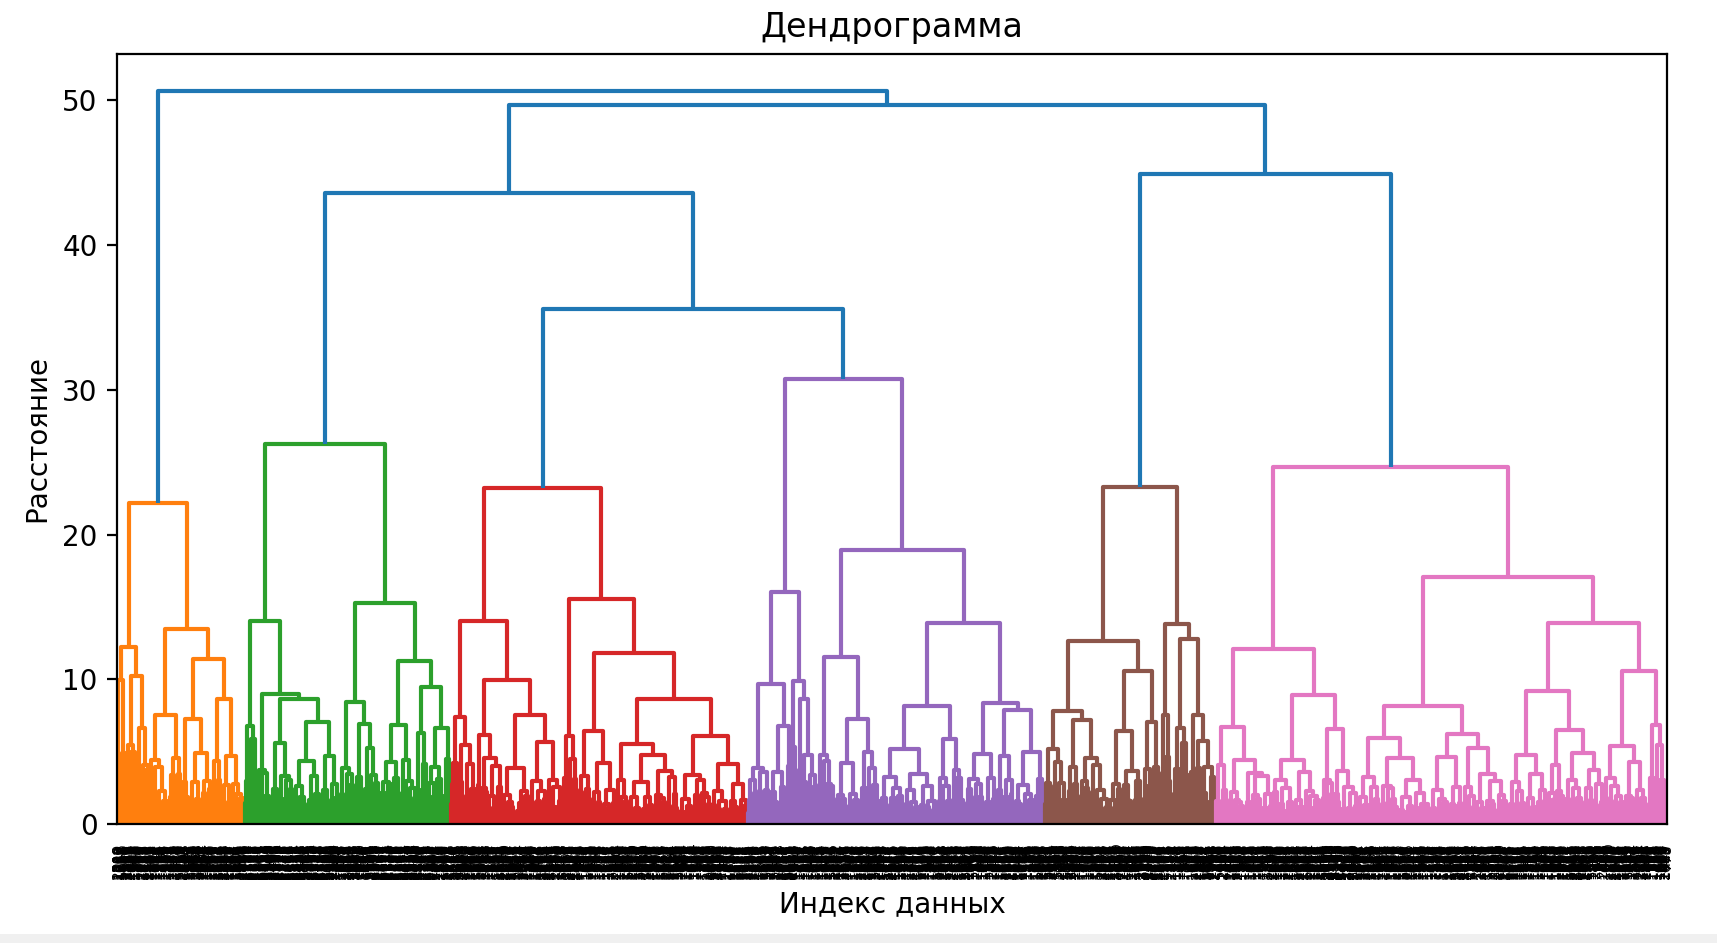
\includegraphics[width=\textwidth]{media/image2.png} % Замените на реальный файл
    \caption{Дендрограмма иерархического кластерного анализа данных}
    \label{fig:dendrogram}
\end{figure}

В таблице 3.10 представлены центры кластеров, построенных методом иерархического кластерного анализа.

\begin{table}[H]
    \centering
    \caption{Координаты центров кластеров, полученных иерархическим методом}
    \label{tab:hier_centers}
    \small
    \begin{tabular}{c|cccccc|c}
        \toprule
        Кластер & PC1 & PC2 & PC3 & PC4 & PC5 & PC6 & Интегр. показ. \\
        \midrule
        1 & -0.1638 & 0.0694  & 0.5357  & -0.1442 & 0.2281  & -0.2943 & 0.0212 \\
        2 & -0.1716 & 0.333   & -0.0001 & -0.1751 & -0.0098 & 1.8352  & 0.1304 \\
        3 & -0.3085 & -0.2686 & -0.8225 & 0.3583  & -0.3612 & -0.0786 & -0.1587 \\
        4 & 2.3393  & 0.0696  & -0.4454 & -0.1347 & -0.1468 & -0.3309 & 0.252 \\
        \bottomrule
    \end{tabular}
\end{table}

В таблице 3.11 предоставлено, каким образом переопределялась нумерация кластеров в зависимости от значений интегрального показателя.

\begin{table}[H]
    \centering
    \caption{Переопределение номеров кластеров (иерархический метод)}
    \label{tab:recode_hier}
    \begin{tabular}{cc}
        \toprule
        Номер кластера (алгоритм) & Номер кластера (интегральный показатель) \\
        \midrule
        4 & 3 \\
        3 & 1 \\
        2 & 2 \\
        1 & 4 \\
        \bottomrule
    \end{tabular}
\end{table}

В таблице 3.12 представлено количество наблюдений в каждом построенном кластере, а также относительная частота этих наблюдений.

\begin{table}[H]
    \centering
    \caption{Количество наблюдений в каждом кластере (иерархический метод)}
    \label{tab:counts_hier}
    \begin{tabular}{ccc}
        \toprule
        Номер кластера & Количество наблюдений & Относительная частота \\
        \midrule
        1 & 200  & 0,0825 \\
        2 & 267  & 0,1101 \\
        3 & 1251 & 0,516 \\
        4 & 706  & 0,2913 \\
        \bottomrule
    \end{tabular}
\end{table}

В таблице 3.13 представлена описательная статистика для интегрального показателя в разрезе полученных кластеров.

\begin{table}[H]
    \centering
    \caption{Описательная статистика для интегральных показателей (иерархический метод)}
    \label{tab:desc_hier}
    \begin{tabular}{c|ccccc}
        \toprule
        Номер кластера & Среднее & Медиана & Минимум & Максимум & Станд. откл. \\
        \midrule
        1 & 0.252  & 0.2131 & -0.31 & 1.19 & 0.2866 \\
        2 & 0.1304 & 0.0902 & -0.49 & 0.94 & 0.2333 \\
        3 & 0.0212 & -0.0103& -0.68 & 0.99 & 0.2292 \\
        4 & -0.1587& -0.1681& -0.6  & 0.4  & 0.1492 \\
        \bottomrule
    \end{tabular}
\end{table}

\subsection{Сравнительный анализ результатов построения статистических кредитных рейтингов}

Таким образом, в первом кластере находятся предприятия с очень высокой платёжеспособностью (кредитоспособностью), во втором --- с платёжеспособностью (кредитоспособностью) выше средней, в третьем --- платёжеспособностью (кредитоспособностью) средней, в четвёртом --- низкой платёжеспособностью (кредитоспособностью).

\clearpage

% ==== ЗАКЛЮЧЕНИЕ ====
\section*{ЗАКЛЮЧЕНИЕ}
\addcontentsline{toc}{section}{ЗАКЛЮЧЕНИЕ}

В курсовом проекте получены следующие основные результаты:
\begin{enumerate}
    \item подготовлен обзор существующих методов анализа финансовой стабильности компаний;
    \item подготовлено описание этапов построения статистических кредитных рейтингов;
    \item построены статистические кредитные рейтинги с помощью двух алгоритмов кластерного анализа и проведена их содержательная интерпретация.
\end{enumerate}

В первом кластере находятся предприятия с очень высокой платёжеспособностью (кредитоспособностью), во втором --- с платёжеспособностью (кредитоспособностью) выше средней, в третьем --- платёжеспособностью (кредитоспособностью) средней, в четвёртом --- низкой платёжеспособностью (кредитоспособностью).

\clearpage

% ==== СПИСОК ИСТОЧНИКОВ ====
\section*{СПИСОК ИСТОЧНИКОВ}
\addcontentsline{toc}{section}{СПИСОК ИСТОЧНИКОВ}

\begin{thebibliography}{99}
\bibitem{1} Малюгин, В.И. Система статистических кредитных рейтингов предприятий: методика построения, верификации и применения / В.И. Малюгин, Н.В. Гринь, П. С. Милевский, А. И. Зубович // Банк. вестн. --- №~11. 2013.
\bibitem{2} Харин Ю. С. Математические и компьютерные основы статистического анализа данных и моделирования : учеб. пособие / Ю. С. Харин, В. И. Малюгин, М. С. Абрамович. --- Мн.: БГУ, 2008.
\bibitem{3} Айвазян, С.А. Межстрановой анализ интегральных категорий качества жизни населения (эконометрический подход) / С.А. Айвазян. --- М.: ЦЭМИ РАН, 2001. --- 61 с. --- (Препринт \# WP/2001/124).
\bibitem{4} Айвазян, С.А. Прикладная статистика. Классификация и снижение размерности / С.А. Айвазян [и др.]. --- М.: Финансы и статистика, 1989. --- 607 с.
\bibitem{5} Ефимова, Ю.В. Методические подходы к оценке кредитоспособности заемщиков // Банковское кредитование. --- №3. --- 2010. --- С. 6--12.
\bibitem{6} Altman E. Financial Ratios, Discriminant Analysis and the Prediction of Corporate Bankruptcy // J. of Finance. --- 1968. --- P. 189--209.
\bibitem{7} Chesser D. Predicting Loan Noncompliance // J. of Commercial Bank Lending. --- 1974. --- August.
\bibitem{8} Fulmer J. [et al.] A Bankruptcy Classification Model for Small Firms // J. of commercial Bank Lending. --- 1984. --- P. 25--37.
\bibitem{9} Ohlson J. A. Financial Ratios and the Probabilistic Prediction of Bankruptcy // Journal of Accounting Research. --- 1980. --- Vol. 18. --- №~1.
\bibitem{10} Beaver W. H. Financial Ratios as Predictors of Failure, Empirical Research in Accounting Selected Studies // Supplement to J. of Accounting Research. --- 1966. --- P. 71--111.
\bibitem{11} Taffler R. J. The assessment of company solvency and performance using a statistical model // Accounting and Business Research. --- 1983. --- P. 295--308.
\bibitem{12} Springate G. Predicting the Possibility of Failure in a Canadian Firm // Unpublished M. B. A. Research Project, Simon Fraser University. --- 1978.
\bibitem{13} Карминский, А.М. Модели корпоративных рейтингов для развивающихся рынков / А.М. Карминский // Корпоративные финансы. --- 2011. --- №~3. --- С. 19--29.
\bibitem{14} Энциклопедия финансового риск-менеджмента /А.А. Лобанов [и др.]; Под. ред. А.А. Лобанова и А.В. Чугунова. --- 2-е изд. --- М.: Альпина Бизнес Букс, 2006. --- 878 с.
\bibitem{15} Карминский, А.М. Рейтинги как мера финансовых рисков: Эволюция, назначение, применение / А.М. Карминский, А.А. Пересецкий // Журн. новой экон. ассоц. --- 2009. --- №~1-2.
\bibitem{16} A Credit Risk Managemenent Framework [Electronic resource]. --- 2003.
\bibitem{17} Crosbie, P. Modelling Default Risk. / P. Crosbie, J. Bohn // Moody's Analytics. --- [Electronic resource] 2003.
\bibitem{18} Савицкая, Г.В. Экономический анализ: Учеб. / Г.В. Савицкая. --- 10-е изд. --- М.: Новое знание, 2008. --- 640 с.
\bibitem{19} Бланк, И.А. Управление финансовыми рисками / И.А. Бланк // К.: Ника-Центр, 2005. --- 600 с.
\bibitem{20} Falcon L.T. Logit Models to Assess Credit Risk / L. T. Falcon // Credit Risk Assessment Revisited. Methodological Issues and Practical Implications. --- European Committee of Central Balance Sheet Data Offices, 2007. --- P. 25--46.
\bibitem{21} Bartlett, M.S. Tests of significance in factor analysis / M.S. Bartlett // British J. Psych. (Statistical Section). --- №3, 1950. --- 77--85 p.
\bibitem{22} Cerny, C.A. A study of a measure of sampling adequacy for factor-analytic correlation matrices /C.A. Cerny, H.F. Kaiser // Multivariate Behavioral Research. --- №12(1), 1977. --- 43--47 p.
\bibitem{23} Малюгин, В.И. Компьютерный анализ данных и моделирование на IBM SPSS / В.И. Малюгин, Н.В. Гринь. --- Мн.: БГУ, 2013.
\end{thebibliography}

\end{document}